\subsection{Industrie 4.0}
Dieses Kapitel soll die Relevanz der Thematik verdeutlichen, indem sie in einen gesellschaftlichen und wirtschaftlichen sowie in einen technischen Kontext gebracht wird. Zunächst wird erläutert, was hinter dem Begriff \textit{Industrie 4.0} steckt. Dem Ausdruck wird mehr Sinn verliehen, wenn die historische Entwicklung bekannt ist. Anschließend werden die treibenden Technologien kurz erläutert. Da die Venetzung für Industrie 4.0 eine tragende Rolle spielt, werden zuletzt Theorien und Technologien zu Kommunikationssystemen aufgegriffen.
\subsubsection{Definition}

Laut der \cite{FraunhoferGesellschaft2016} habe die \textit{Industrie 4.0} einen revolutionären Einfluss auf die Wertschöpfung in der Industrie und somit auf die Volkswirtschaft. Dieser Marketingbegriff prägt heute die Agenda vieler Unternehmen und Forschungseinrichtungen. Doch was genau hinter dem Begriff zu verstehen ist, bleibt aufgrund des Fehlens einer  \glqq wissenschaftlichen Präzision\grqq{} uneindeutig \citep{Bendel2019}. Für die Gestaltung der digitalen Transformation entstand das Netzwerk \textit{Plattform Industrie 4.0} zwischen der Bundesregierung, Forschungseinrichtungen und Wirtschaft. Dieses hat zum Ziel, die Produktion mittels modernster Informations- und Kommunikationstechnologien entlang der Wertschöpfungkette \glqq flexibler, individueller und effizienter\grqq{} gestalten \citep{BWE2019}. In der Umsetzungstrategie der \citet[S. 8]{BITKOM2015} wird der Begriff wie folgt definiert:

\begin{displayquote} \glqq Der Begriff Industrie 4.0 steht für die vierte industrielle Revolution, einer neuen Stufe der Organisation und Steuerung der gesamten Wertschöpfungskette über den Lebenszyklus von Produkten. Dieser Zyklus orientiert an den zunehmend individualisierten Kundenwünschen und erstreckt sich von der Idee, dem Auftrag über die Entwicklung und Fertigung, die Auslieferung eines Produkts an den Endkunden bis hin zum Recycling einschließlich der damit verbundenen Diensleistungen.\grqq{}
\end{displayquote}

Darüber, auf welcher Basis die digitale Transformation in der Industrie stattfinden wird, scheinen sich jedoch alle einig: durch die \textit{intelligente Vernetzung aller am Produktlebenszyklus beteiligten Menschen, Objekte und Systeme} \citep{Roth2016}. Das Wesentliche der Vernetzung bilden dezentrale \acf{cpss} \citep{Bendel2019a}. Die tatsächliche Wertschöpfung ergibt sich aus den in Echtzeit verfügbaren quantitativen Informationen, aus welchen man durch Analysen qualitative Erkenntnisse schließen und optimierte Aktionen auslösen kann \citep{Hnisch2017}. Nach \cite{Sendler2016} gibt es für den Erfolg von \textit{Industrie 4.0} entscheidende Faktoren: Mittlerweile sind digitale Komponenten wie Sensoren, Aktoren oder Kameras so günstig und klein, dass sie in allen möglichen Bereichen eingebaut werden und Umgebungsdaten messen und aufnehmen können. Dank dem Internetprotokoll IPv6 und dem dadurch verfügbaren Adressraum können diese Komponenten ihren Platz im Internet finden. Dass die Informatik sich damit zur wichtigsten Ingenieursdisziplin entwickle, sei unterlässlich, da sie für die Vernetzung der Welt gebraucht werde.

\subsubsection{Historischer Kontext}

Um den aktuellen Stellenwert von Industrie 4.0 zu beschreiben, wird oft von der vierten industriellen \textit{Revolution} gesprochen. Revolutioniert wurde die Industrie erstmalig im 18. Jahrhundert mit der Erfindung der Dampfmaschine durch Thomas Newcomon und James Watt - die \textbf{erste industrielle Revolution} \citep{Roth2016}. Mit Errungenschaften wie dem dampfgetriebenen Webstuhl ging eine \textbf{Mechanisierung }der Produktion einher. Schon damals förderte eine Erfindung, die Lokomotive, eine Vernetzung, die einen regen Warenaustausch ermöglichte \citep{Barthelmaes2017}.

Durch die \textbf{Elektrifizierung} in der Industrie und der Zerlegung von Produktionsschritten in einzelne Einheiten konnten ab 1870 die Waren auf Fließ- und Förderbändern in Massen produziert werden. Angestoßen wurde die \textbf{zweite industrielle Revolution} von Erfindungen wie der Verbrennungskraftmaschine und dem Elektromotor sowie der Herstellung von Syntheseprodukten. Neben fossilen Energieträgern wie Kohle und Öl kam auch die Kernkraft hinzu \citep{Barthelmaes2017}.


Die \textbf{dritte industrielle Revolution} ab den 1970er Jahren, in der wir uns noch heute befinden,  brachte die \textbf{Automatisierung} der Produktion durch die \textbf{Digitalisierung} \citep{Voigt2018}. Getrieben wurde die Revolution durch das Wirtschaftswunder der 1960er Jahre \citep{Roth2016} und ermöglicht durch den Ausbau von Informations- und Kommunikationstechnologien. Entscheidende Technologien waren vielfältig. 1941 entwickelte der Bauingenieur Konrad Zuse den ersten programmgesteuerten und vollautomatischen Computer und setzte den Grundstein für eine rasante Entwicklung der nachfolgenden Technologien. Mit der Vebreitung von Mikroprozessoren, der Miniatisierung der Elektronik sowie der nach dem Mooreschen Gesetz vorausgesagten Zunahme der Prozessorstärke nahm die Welt ein neues Tempo an \citep{Sendler2016}. Einen nicht unwesentlichen Beitrag leistet die Raumfahrtechnik, ohne deren Satellitentechnik eine globale Kommunikation nicht möglich wäre. Da der energieintesive Einsatz dieser Technologien ein Bewusstsein über die Endlichkeit der fossilen Ressourcen schuf, kamen auch erneuerbare Energien hinzu \citep{Barthelmaes2017}.

\begin{figure}[ht]
  \centering
  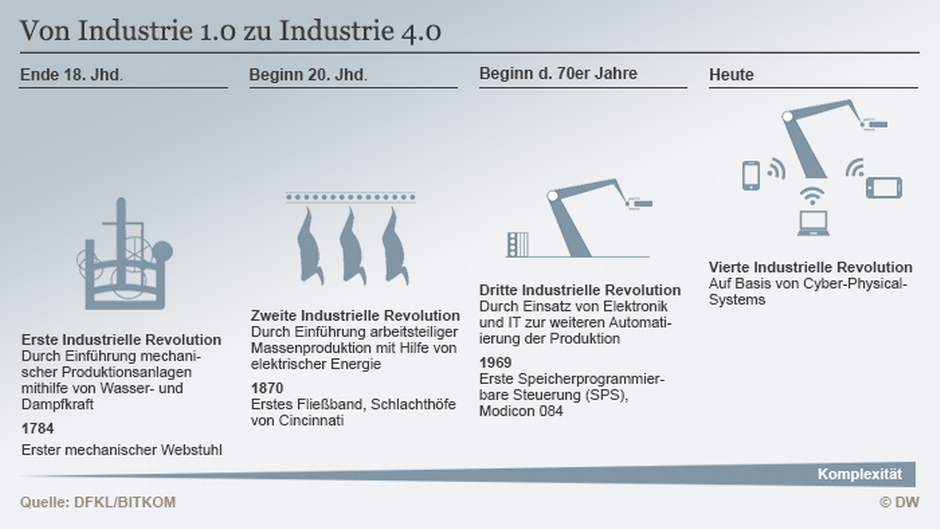
\includegraphics[width=1.0\linewidth]{industrie_40_revolution.png}
  \caption[Die vier Stufen Industrieller Revolutionen]{Die vier Stufen Industrieller Revolutionen \citep[S. 9]{Bauer2014}}
  \label{fig:revolutions}
\end{figure}

Die Industrie 4.0 tatsächlich als \textbf{vierte Industrielle Revolution} zu bezeichnen wird kritisiert, da sie u.a. keine neuen technologischen Innovationen hervorbringe, sondern sich lediglich an den Technologien der dritten Revolution bediene \citep{Barthelmaes2017}. Auch wenn die Technologien nicht unbedingt als revolutionär zu bezeichnen sind, durchlaufen sie eine Evolution und stoßen einen Wandel durch Industrie 4.0 an \citep{Roth2016}. Es entstehen eine Vielzahl neuer Geschäftsmodelle und Produktionsprozesse, die zu Effizienz- und Produktivitätssteigerungen führen \citep{BITKOM2015}.


\subsubsection{Technologische Treiber}\label{technologien}

Industrie 4.0 zeichnet sich durch das Zusammenwachsen der realen und physischen Welt zu mit Sensorik und Aktorik ausgestatten Objekten aus, die per Internet miteinander verbunden sind \citep{BITKOM2015}. Dieses Phänomen ist geprägt von Trendtechnologien wie \textit{Big Data, Internet of Things, Blockchain, Cloud Computing und Machine Learning}, die in kombinierter Nutzung einen Mehrwert erzeugen.
\paragraph{\acf{cpss}}
sind physische Objekte mit einem Datenobekt als virtuelle Präsenz im Netz und bilden die Grundlage von Industrie 4.0 \citep{Drath2016}. Das Hauptmerkmal eines \ac{cpss} ist das mit dem Internet verbundene \textit{eingebettete System}, welches über Sensoren Daten aus der Umwelt aufnimmt, über Aktoren wieder mit ihr interagiert und sich somit an sie anpasst. Diese Fähigkeit, die Informationen zu verarbeiten und zu versenden, wird dem \ac{cpss} durch \textit{Ubiquitous Computing} verliehen. Entscheidend für die implizite und allgegenwärtige Nutzung von IT  ist neben der Austattung mit Sensoren und Aktoren die Verfügbarkeit von Kommunikationsmodulen und Rechenleistung \citep{Roth2016}. Somit wird den Systemen die Fähigkeit verliehen, sich untereinander \textit{dezentral und autonom} zu vernetzen \citep{Bauernhansl2014}. Zudem besitzen \ac{cpss} die Eigenschaft, auch mit Menschen zu interagieren: zum einen über direkte Kommunikation wie Monitoring und Befehle und zum anderen, um komplexe Aufgaben gemeinsam zu lösen \citep{Lueth2016}.


\begin{figure}[ht]
  \centering
  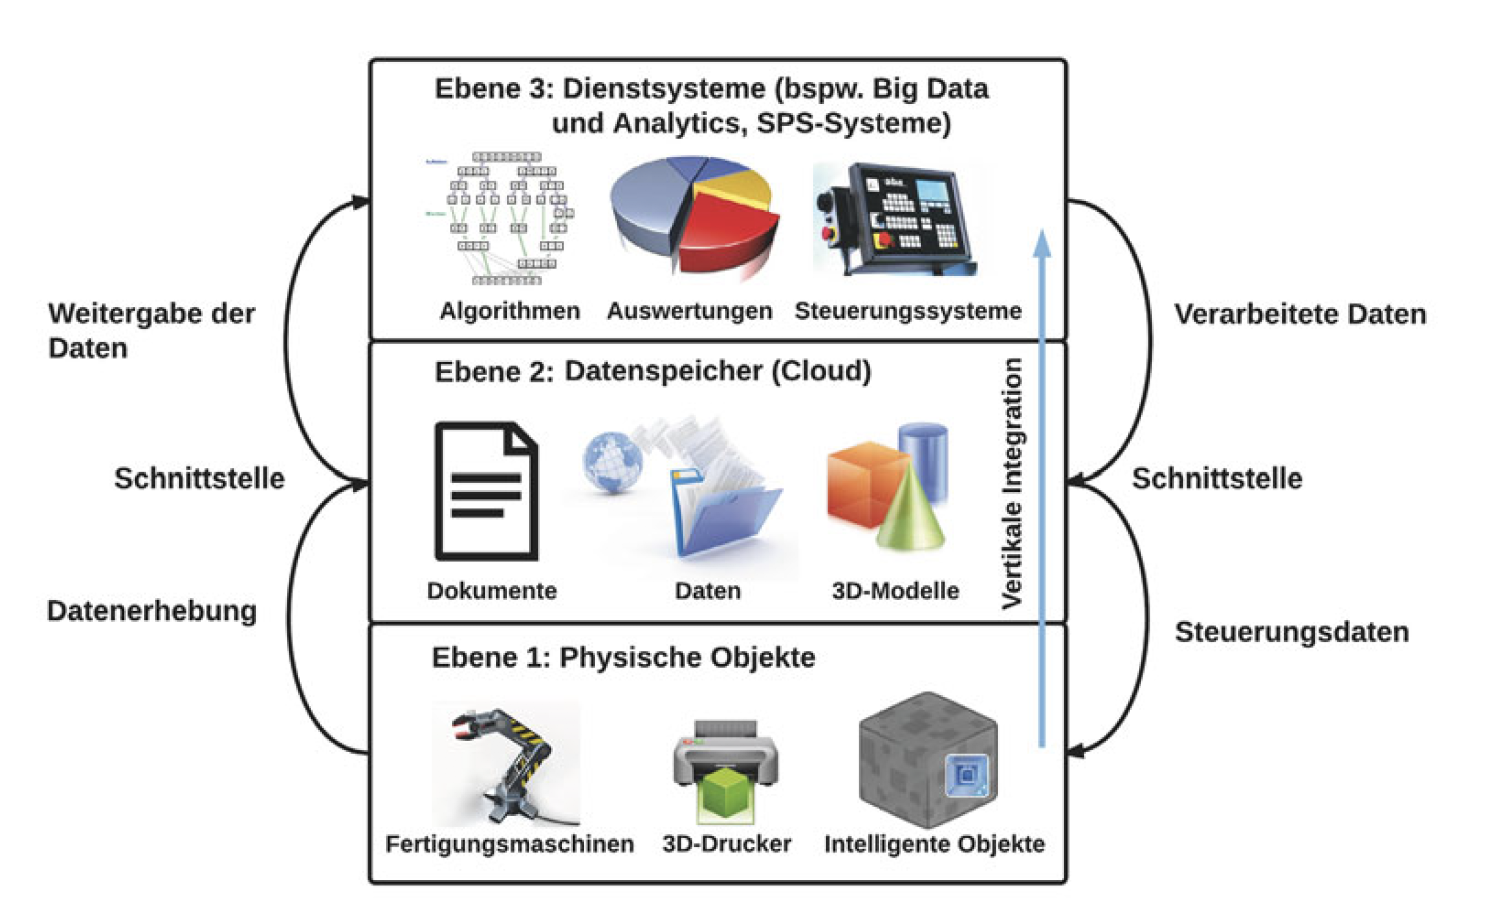
\includegraphics[width=1.0\linewidth]{CPS.png}
  \caption[CPS in der Industrie 4.0]{\ac{cpss} in der Industrie 4.0 \citep[S. 30]{Roth2016}}
  \label{fig:cpskreis}
\end{figure}

\paragraph{Das \acf{iot}} ist das Verbindungsstück zwischen dem Internet und dem Objekt des \textit{Ubiquitous Computing} \citep{Roth2016}. Das Gerät bzw. das \textit{Thing} ist in der Lage dazu, selbstständig den eigenen Zustand zu erfassen und zu kommunizieren \citep{Kenn2016}. Dafür muss das Gerät allerdings eindeutig mit z.B. IP-Adressen oder \ac{rfid} identifizierbar sein. Während das \acf{ipv4} mit seinen rund 4,3 Milliarden Adressen noch nicht einmal die in 2016 verbundenen 6 Milliarden Geräte (siehe Abbildung \ref{fig:connecteddevices}) platzieren kann, schafft das \ac{ipv6} mit 340 Sextillionen (2 hoch 128) Adressen genügend Platz für 20 Milliarden prognostizierte Geräte in 2020. Das Entscheidende für das \textit{Internet} der Dinge ist, dass die Daten nicht lokal auf dem Gerät gespeichert werden, sondern über das Dienste im Internet bestimmten Personen oder Parteien zur Verfügung gestellt werden: \textbf{das Internet der Dinge und Dienste} \citep{Hanisch2017}. Einen Mehrwert bilden die Daten durch die zentrale Aggregation und Analyse, auf deren Grundlage Entscheidungen getroffen werden können. Diese Eigenschaften lassen sich in der für \ac{iot}-Projekte typische Grundarchitektur wiederfinden: \textit{Datentransport, Datenhaltung und Analyse} \citep{Kenn2016}. Der Kreis schließt sich durch die Weitergabe der verarbeiteten Daten als Steuerungsdaten an die Maschine, sodass sich der Fokus von einer Mensch-Maschinen-Interaktion auf eine Maschine-zu-Maschine-Interaktion verschiebt  (s. Abbildung \ref{fig:cpskreis}).

\begin{figure}[ht]
  \centering
  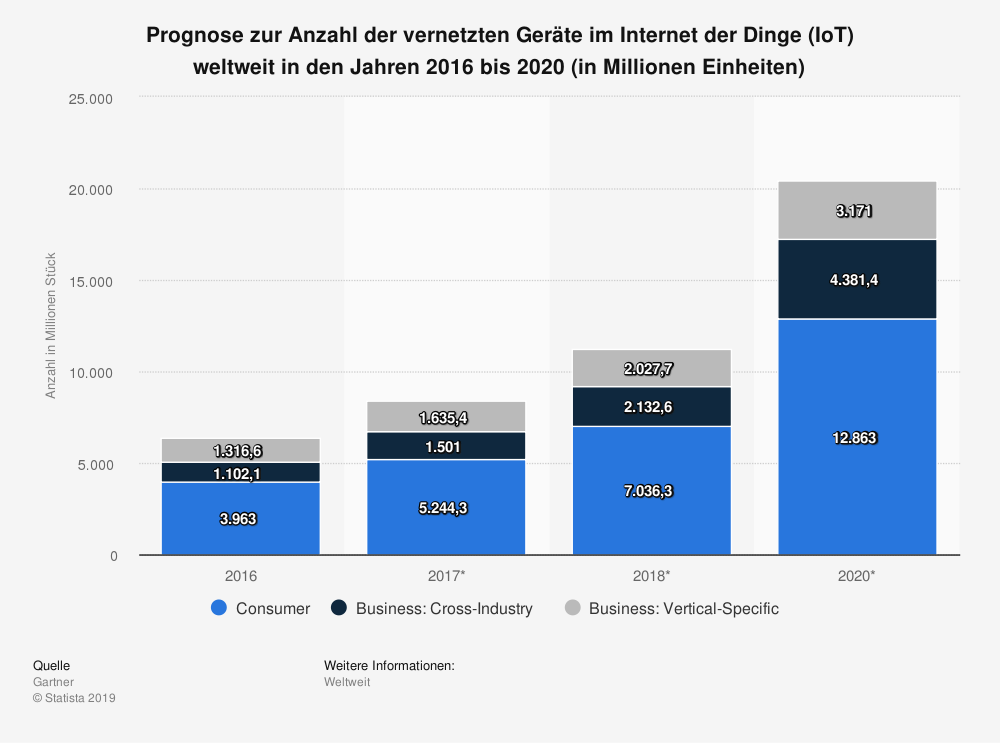
\includegraphics[width=1.0\linewidth]{statistic_connecteddevices.png}
  \caption[Prognose zur Anzahl der vernetzten Geräte im Internet of TThings weltweit]{Prognose zur Anzahl der vernetzten Geräte im \ac{iot} weltweit \citep{Gartner2017a}}\label{fig:connecteddevices}
\end{figure}

\paragraph{Cloud Computing} stellt die IT-Infrastruktur, die ein Industrie 4.0-fähiges \ac{cpss} benötigt. Der \textit{Datentransport} vom Gerät hat oftmals eine Cloud-Plattform als Ziel, auf der die \textit{Datenhaltung} stattfindet \citep{Elsner2018}. Die in die Cloud auslagerbaren Dienste wie Big Data oder Analytics ermöglichen \textit{Analysen} durch Aggregationen und Auswertungen \citep{Roth2016}. Der Nutzen der Cloud steigert sich durch das Kombinieren der Angebote der Cloud-Dienstleister wie Amazon, SAP oder Microsoft \citep{Hnisch2017}. Diese Anbieter stellen besitzen weltweit Rechenzentren, auf denen für Industrie 4.0 ausschlaggebende Services bereitgestellt werden:

\noindent\hspace*{10mm}
 \textbf{Big-Data-Technologien} dienen der Verarbeitung der in massiven Mengen gesammelten Daten und ermöglichen damit die Nutzung, Verwertung, Vermarktung und vor allem Analyse der digitalen Daten \citep{Radtke2019}. Die Datenmengen können z.B. aus Maschine-zu-Maschine Interaktionen, Transaktionen, Verbraucherdaten oder sozialen Medien stammen \citep{Elsner2018}.

 \noindent\hspace*{10mm}
 \textbf{Machine Learning} beruht sich ähnlich wie Big Data auf die \textit{Extraktion von Wissen aus Daten} und ermöglicht dem Computer die selbstständige Ausführung bestimmter Aufgaben, ohne dass sie explizit programmiert werden müssen \citep{Hnisch2017}. Mittels Algorithmen können die Programme aus den Daten lernen und Muster erkennen, aus denen sie Schlussfolgerungen ziehen können \citep{Elsner2018}. Somit könne Aussagen über das wahrscheinlich zukünftige Verhalten des Systems getroffen werden (\textit{Predictive Analytics}), aus denen in Zukunft auch Handlungsoptionen vorgeschlagen werden sollen (\textit{Prescriptive Analytics}) \citep{Huebschle2017}.

 \noindent\hspace*{10mm}
 \textbf{Blockchain} ist die Technologie, auf der die erste Kryptowährung Bitcoin basiert. Die Haupteigenschaften der digitalen Währung sind die Dezentralität sowie  die Unveränderbarkeit und Transparenz der Transaktionshistorie. Auf Grundlage dieser Eigenschaften eines Peer-to-Peer-Systems entwickeln sich neue Geschäftsmodellmuster in verschiedensten Branchen wie Finanzen,  Logistik und Transport, aber auch neue Sicherheitskonzepte \citep{Elsner2018}.

\subsubsection{Kommunikationssysteme}

Die Vernetzung ist der Schlüssel zur Dezentralität und Autonomie der \ac{cpss} - und somit zum Erfolg - in der Industrie 4.0 \citep{Bauernhansl2014}. 1980 stellte der Erfinder des Ethernets Robert Meltcafe eine Theorie zum Nutzen eines Netzwerks auf, die mit dem sog. \textit{Netzwerkeffekt} in vielen wissenschaftlichen Disziplinen Anwendungen findet \citep{Lea2018}. \citet[S. 18]{Bauernhansl2014} beschreibt das Konzept, \glqq [...] dass der Nutzen eines Kommunikationssystems mit dem Quadrat der Anzahl seiner Teilnehmer wächst.\grqq{} Angewandt auf das \acf{iot} stellen die Sensoren und Edge-Geräte die Nutzer dar und steigern den Wert der \ac{cpss}, welche die Kommunikationssysteme bilden \citep{Lea2018}. Dem rasanten Anstieg der  miteinander vernetzten Geräte (s. Abbildung \ref{fig:connecteddevices}) liegt außerdem das nach wie vor geltende Moore'sche Gesetz zugrunde \citep{Barthelmaes2017}. Demnach verdoppelt sich die Rechner- bzw. Chipleistung alle zwei Monate bei gleichbleibenden Preisen. Folglich können Technologien, die aktuelle noch zu hohe Preise aufweisen, in Zukunft günstiger betrieben werden \citep{Bauernhansl2014}. Dieser Zusammenhang fördert die Fähigkeiten zur autonomen und intelligenten Vernetzung der dezentralen Systeme und führt zur Effizienzsteigerung \citep{Barthelmaes2017}.
\\\\
Flexibilität in der Vernetzung bieten standardisierte und simple Protokolle wie \ac{rest} und \ac{mqtt} zum Datenaustausch im Internet \citep{Hnisch2017}.

\textbf{\ac{rest}} ist ein Architekturstil, der auf dem \ac{http} basiert und zum Lesen, Erstellen und Bearbeiten von Ressourcen dient. Der Ansatz ist, einheitliche Anfragen an die Ressourcen-Schnittstellen per \ac{uri} zu adressieren und \ac{http}-kodiert zu versenden \citep{Sendler2016}.

\textbf{\ac{mqtt}} ist ein offenes Kommunikationprotokoll, welches zur Übertragung von Telemetriedaten zwischen Maschinen bei niedriger Bandbreite geeignet ist und basiert auf dem Publisher-Subscriber-Prinzip \citep{Lea2018}.
\begin{itemize}
  \item OPCUA
\end{itemize}
